\documentclass[conference]{IEEEtran}
\usepackage[UTF8]{ctex}


\title{Study on 'Distributed Compressive Sensing'}
\author{Huang, Dongbo}


\usepackage{amsmath}
\usepackage{amsthm}
\usepackage{amssymb}
\usepackage{amsfonts}
\usepackage{pgfplots}
\usepackage{graphicx}

\bibliographystyle{IEEEtran}



\begin{document}
	
	
\theoremstyle{plain} \newtheorem{theorem}{Theorem}
\newtheorem{remark}{Remark}
\maketitle
\today



\begin{abstract}
学习笔记
\end{abstract}

\section{Introduction}
This paper is a continuing work of \ldots.
\section{discrete noiseless systems}
\subsection{The Discrete Noiseless Channel}
\subsection{The Discrete Source of Information}
\subsection{The Series of Approximations to English}
\subsection{Graphical Representation of a Markoff Process}
\subsection{Ergodic and Mixed Sources}
\subsection{Choice, Uncertainty and Entropy}
\subsection{The Entropy of An Information Source}


\subsection{Representation of The Encoding and Decoding Operations}
%\theoremstyle{plain} \newtheorem{theorem}{Theorem}
\begin{theorem}
The output of a finite state transducer driven by a finite state statistical source is a finite state statistical source, with entropy(per unit time) less than or equal to that of the input. If the transducer is non-singular they are equal.
\end{theorem}
\begin{theorem}
Let the system of constraints considered as a channel have a capacity$C= logW$. If we assign
\[ p_{ij}^{(s)}=\dfrac{B_{j}}{B_{i}}W^{-\ell_{ij}^{(s)}} \]
where $ell_{ij}^{(s)}$ is the duration of the $s^{th}$ symbol leading from state i to state j and the $B_{i}$ satisfy
\[B_{i}=\sum_{s,j} B_{J}W^{-\ell_{ij}^{(s)}}\]
then H is maximized and equal to C
\end{theorem}
By proper assignment of the transition probabilities the entropy of symbols on a channel can be maximized at the channel capacity.


\subsection{The Fundamental Theorem For a Noiseless Channel}
\begin{theorem}
Let a source have entropy H bits per symbol and a channel have a capacity C bits per second. Then it is possible to encode the output of the source in such a way as to transmit at the average rate $\frac{C}{H}-\epsilon$
symbols per second over the channel where is arbitrarily small. It is not possible to transmit at an average rate greater than$\frac{C}{H}$.
\end{theorem}

The high probability group is coded in an arbitrary one-to-one way into this set. The remaining sequences are represented by larger sequences, starting and ending with one of the sequences not used for the high probability group.

The average number $H^{'}$ of binary digits used per symbol of original message is easily estimated. We have

\[
H^{'}=\dfrac{1}{N}\sum_{} m_{s}p_{s} = 0
\]
But,
\[
\dfrac{1}{N}\sum_{}(log_{2}\dfrac{1}{p_{s}})p_{s} \le \dfrac{1}{N}\sum_{} m_{s}p_{s} < \dfrac{1}{N}\sum_{} (1+log_{2}\dfrac{1}{p_{s}})p_{s}
\]
and therefore,
\[ G_{N}\le H^{'}<G_{N}+\dfrac{1}{N} \]
As $N$ increases $G_{N}$ approaches $H$, the entropy of the source and $H^{'}$ approaches $H$.
The percent excess time needed over the ideal is therefore less than
\[ \dfrac{G_{N}}{H}+\dfrac{1}{HN}-1\]

\subsection{Discussion and Examples}

\section{The Discrete Channel With Noise}
\subsection{Representation of A Noisy Discrete Channel}
If a particular transmitted signal always produces the same received signal, i.e., the received signal is a definite function of the transmitted signal, then the effect may be called distortion.

If this function has an inverse -- no two transmitted signals producing the same received signal -- distortion may be corrected, at least in principle, by merely performing the inverse functional operation on the received signal.
\[
p_{\alpha,i}(\beta,j),
\]
is the probability, if the channel is in state $\alpha$ and symbol $i$ is transmitted, that symbol $j$ will be received and the channel left in stat $\beta$. Thus $\alpha$ and $\beta$ range over the possible states, $i$ over the possible transmitted signals and $j$ over the possible received signals.

In the noiseless case $H(y) = H(x)$. And
\[H(x,y)=H(x)+H_{x}(y)=H(y)+H_{y}(x)\]
All of these entropies can be measured on a per-second or a per-symbol basis.
\subsection{Equivocation and Channel Capacity}

The proper correction to apply to the amount of information transmitted is the amount of this information which is missing in the received signal, or alternatively the uncertainty when we have received a signal of what was actually sent.



The rate of actual transmission, $R$, would be obtained by subtracting from the rate of production (i,e., the entropy of the source) the average rate of conditional entropy.
\[R=H(x)-H_{y}(x)\]
The conditional entropy $H_{y}(x)$ will, for convenience, be called
the $equivocation$
(条件信息量总平均值、存疑度、模糊). It measures the average ambiguity of the received signal.

If a 0 is received the a $a posterior$ probability that a 0 was
transmitted is 0.99, and that a 1 was transmitted is 0.01. These
figures are reversed if a 1 is received. Hence

\begin{align*}
	H_{y}(x) & = -[0.99log0.99 + 0.01log0.01] \\
	         & =0.081 bits/symbol
\end{align*} or 81 bits per second. We may say that the system is transmitting at a rate 1000-81 = 919 bits per second. In the extreme case where a 0 is equally likely to be received as a 0 or 1 and similarly for 1, the a posteriori probabilities are 12, 12 and
\begin{eqnarray*}
	H_{y}(x) &=& -[\dfrac{1}{2}log\dfrac{1}{2}+\dfrac{1}{2}log\dfrac{1}{2}]\\
	%&= 1\ bit\ per\ symbol
			 &=& 1\ bit/symbol
\end{eqnarray*} or 1000 bits per second. The rate of transmission is then 0 as it should be.

\begin{theorem}
	If the correction channel has a capacity equal to  $H_{y}(x)$ it is possible to so encode the correction data as to send it over this channel and correct all but an arbitrarily small fraction $\epsilon$of the errors. This is not possible if the channel capacity is less than $H_{y}(x)$.
\end{theorem}
粗略地说,$ H_{y}(x) $是在接收端用每秒来正确译码所必需的额外信息。文中公式$ H_{y}(x,z)\geq H_{y}(x)$由于:
\begin{align*}
	H_{y}(z)+H_{yz}(x)     & = H(x,y,z)-H(y)              \\
	                       & \&\ \ \ \ \ \ \              \\
	H_{y}(x,z)             & = H(x,y,z)-H(y)              \\
	                       & \Rightarrow                  \\
	H_{y}(z)+H_{yz}(x)     & \geq H_{y}(x)                \\
	                       & and :                        \\
	H_{yz}(x)\geq H_{y}(x) & -H_{y}(z) \geq H_{y}(x)-H(z)
\end{align*}
有噪信道的信道容量应该等于传输率的最大值。因此信道容量为:
\[
C=Max(H(x)-H_{y}(x))
\]
在无噪信道中,$H_{y}(x)=0$。

\subsection{The Fundamental Theorem for A Discrete Channel with Noise}
很明确的是,当信息以带有冗余的形式进行传输时,错误概率会降低。因此可能会这样认为,为了使得错误概率趋近于0,则编码冗余必须无限长,因此传输速率也趋近于0。事实绝非如此。如果如以上所假设:则不能得到一个明确的容量,只能得到一个指定错误发生频率或者指定的不确定度下的容量;当抗扰要求更要的时候信道容量也会下降。

Actually the capacity $C$ defined above has a very definite significance.It is possible to send information at the rate $C$ through the channel $with as small a frequency of errors or equivocation as desired$ by proper encoding. 实际上以上信道容量C的定义有一个十分明确的重要意义。通过适当的编码方法,可以使信息以一个预期小的错误或模糊度频率,码率为C在信道中进行传输。而当码率大于C时,则不能成立。If an attempt is made to transmit at a higher rate than C, say C R1, then there will necessarily be an equivocation equal to or greater than the excess R1.
%\begin{tikzpicture}
%\begin{axis}
%\addplot[color=red]{exp(x)};
%\end{axis}
%\end{tikzpicture}
%%Here ends the furst plot
%\hskip 5pt
%%Here begins the 3d plot
%\begin{tikzpicture}
%\begin{axis}
%\addplot3[
%surf,
%]
%{exp(-x^2-y^2)*x};
%\end{axis}
%\end{tikzpicture}

\begin{theorem}
	Let a discrete channel have the capacity C and a discrete source the entropy per second H. if $H \leq C $there exists a coding system such that the output of the source can be transmitted over the channel with an arbitrarily small frequency of errors(or an arbitrarily small equivocation). if $H>C$ it is possible to encode the source so that the equivocation is less than $H-C+\epsilon$ where $\epsilon$ is arbitrarily small. There is no method of encoding which gives an equivocation less than $H-C$.
\end{theorem}
There are $2_{TR}$ messages distributed at random in $2_{TH(x)}$ points. The probability of a particular point being a message is thus
\begin{align*}
2^{T(R-H(x))}
\end{align*}

The probability that none of the points in the fan is a message (apart from the actual originating message) is
\begin{align*}
P=[1-2^{T(R-H(X))}]^{2^{TH_y(x)}}.
\end{align*}
Now $R<H(x)-H_y(x)$ so $R-H(x)=-H_y(x)-\eta$ with $\eta$ positive. Consequently
\begin{align*}
P=[1-2^{-TH_y(x)-T \eta }]^{2^{TH_y(x)}}
\end{align*}
approaches (as $T \longrightarrow \infty $)
\[
1-2^{-T\eta}
\] 
Hence the probability of an error approaches zero and the first part of the theorem is proved.

The last statement of the theorem is a simple consequence of our definition of $C$. Suppose we can encode a source with $H(x)=C+a$ in such a way as to obtain an equivocation $H_y(x)=a-\epsilon$ with $\epsilon$ positive. The 
\begin{align*}
R=H(X)		&=C+a		\\
and						\\
H(x)-H_y(x)	&=C+\epsilon
\end{align*}
with $\epsilon$ positive. This contradicts the definition of $C$ as the maximum of $H(x)-H_y(x)$.

%\begin{figure}
%%\centering
%\center{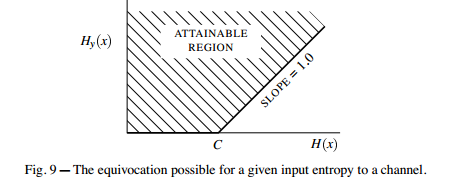
\includegraphics[width=0.7\linewidth]{figures/figure1}}
%\caption{}
%\label{fig:figure1}
%\end{figure}
\subsection{Discussion}
\begin{theorem}
	$ \lim_{n\to\infty}\dfrac{logN(T,q)}{T}=C$, where C is the channel capacity, provided that q does not equal 0 or 1.
\end{theorem}

换言之,无论我们如何设置可靠性的界线,当时间T足够大时,我们都可以在T时间内在相应的$CT bits$中可靠区分出足够的信息。

\subsection{Example of A Discrete Channel and Its Capacity}
To let C maximized, $H(x)-H_y(x)$ must be maximized, and $P+2Q=1$, it is considered:
\begin{equation*}
U = -PlogP-2QlogQ-2Q\alpha+\lambda(P+2Q)
\end{equation*}
in order to eliminate $\lambda$, we calculate the partial differentiation:
\begin{equation*}
\begin{gathered}
\dfrac{\partial U}{\partial P}=-1-logP+\lambda=0 \\
\dfrac{\partial U}{\partial Q}=-2-2logQ-2\alpha+2\lambda=0 \\
\Longrightarrow \\
logP=logQ+\alpha
P=Qe_{\alpha}=Q\beta \\
and \\
P+2Q=1 \\
\Longrightarrow \\
P=\frac{\beta}{\beta+2},Q=\frac{1}{\beta+2}\\
use\ P,\ Q\ in\ U\ and\ \Longrightarrow\\
C=log\frac{\beta+2}{\beta}
\end{gathered}
\end{equation*}




\section{MATHEMATICAL PRELIMINARIES}

In this section the case where the signals or message or both are continuously variable is considered. To a considerable extent the continuous case can be obtained through a limiting process from the discrete case by \emph{\textbf{dividing the continuum of messages and signals into a large but finite number of small regions and calculating the various parameters involved on a discrete basis}}. A preliminary study, however, indicates that the theory can be formulated in a completely axiomatic and rigorous manner which includes both the continuous and discrete cases and many others. The occasional liberties taken with limiting processes in the present analysis can be justified in all cases of practical interest.

\subsection{Sets and Ensembles of Functions}
An ensemble of functions $f_{\alpha}(t)$ is \emph{\textbf{stationary}} if the same ensemble results when all functions are shifted any fixed amount in time. The ensemble
\begin{equation*}
f_{\theta}(t)=sin(t+\theta)
\end{equation*}
is stationary if $\theta$ is distributed uniformly from $0$ to $2\pi$. If we shift each function by $t_1$ we obtain
\begin{align*}
f_{\theta}(t+t_1) &= sin(t+t_1+\theta)
&=sin(t+\varphi)
\end{align*}
with $\varphi$ distributed uniformly from $0$ to $2\pi$. Each function has changed but the ensemble as a whole is invariant under the translation. The other examples given above are also stationary.

An ensemble is \emph{ergodic} if it is stationary, and there is no subset of the functions in the set with a probability different from 0 to 1 which is stationary. The ensemble
\begin{equation*}
sin(t+\theta)
\end{equation*}
is ergodic. No subset of these functions of probability$ \neq 0,1 $is transformed into itself under all time translations. On the other hand the ensemble
\begin{equation*}
asin(t+\theta)
\end{equation*}
with $a$ distributed normally and $\theta$ uniform is stationary but not ergodic. The subset of these functions with $a$ between 0 and 1 for example is stationary.

\section{THE CONTINUOUS CHANNEL}


\bibliography{IEEEabrv, ref}
\end{document}



